\hypertarget{group__sys__prot}{}\section{Critical sections}
\label{group__sys__prot}\index{Critical sections@{Critical sections}}
Collaboration diagram for Critical sections\+:
\nopagebreak
\begin{figure}[H]
\begin{center}
\leavevmode
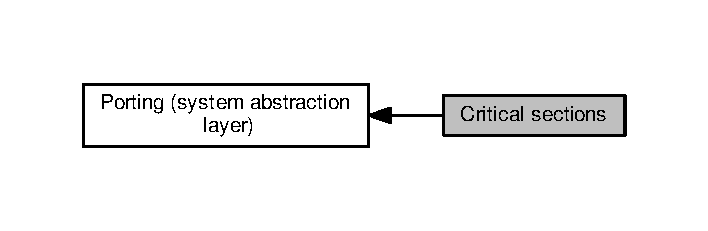
\includegraphics[width=340pt]{group__sys__prot}
\end{center}
\end{figure}
Used to protect short regions of code against concurrent access.
\begin{DoxyItemize}
\item Your system is a bare-\/metal system (probably with an R\+T\+OS) and interrupts are under your control\+: Implement this as Lock\+Interrupts() / Unlock\+Interrupts()
\item Your system uses an R\+T\+OS with deferred interrupt handling from a worker thread\+: Implement as a global mutex or lock/unlock scheduler
\item Your system uses a high-\/level OS with e.\+g. P\+O\+S\+IX signals\+: Implement as a global mutex 
\end{DoxyItemize}